\documentclass[12pt,a4paper]{book}
\usepackage[utf8]{inputenc}
\usepackage[portuguese]{babel}
\usepackage[T1]{fontenc}
\usepackage{geometry}
\usepackage{graphicx}
\usepackage{setspace}
\usepackage{subcaption}


\newcommand{\nomesoftware}{AWGApp}

% Definindo as margens
\geometry{
 a4paper,
 margin=3cm
}

\title{\nomesoftware: Manual do Usuário}
\author{Felipe Walter Dafico Pfrimer}
\date{\today}

\begin{document}

\maketitle

\tableofcontents

\doublespacing  % Aplica espaçamento duplo em todo o documento
\chapter*{Introdução}
\addcontentsline{toc}{chapter}{Introdução}

Este manual tem como objetivo fornecer uma visão abrangente das funcionalidades e da utilização do \textbf{\nomesoftware}, um aplicativo versátil e inovador projetado para atender às necessidades de usuários interessados em geração e manipulação de formas de onda e controle de dispositivos via \textit{Bluetooth}.

O \textbf{\nomesoftware} destaca-se por sua capacidade de gerar diferentes tipos de formas de onda, como triangular, senoidal e quadrada, permitindo ao usuário explorar uma ampla gama de frequências, amplitudes e outras configurações específicas. Além disso, o aplicativo oferece uma funcionalidade robusta de manipulação de pontos, que permite a organização e análise detalhada dos dados gerados.

Com uma interface intuitiva e fácil de usar, o \textbf{\nomesoftware} é adequado tanto para profissionais da área técnica como para entusiastas e estudantes que buscam uma ferramenta eficiente para estudos e projetos relacionados à eletrônica e ao controle de dispositivos.

Este manual irá guiá-lo através das principais características do aplicativo, oferecendo instruções detalhadas sobre como maximizar seu uso e aproveitar todas as funcionalidades disponíveis.

% Aqui vão os outros capítulos e seções do manual

\chapter{Configuração e Instalação}

Este capítulo fornece instruções detalhadas para a instalação do \textbf{\nomesoftware{}} em dispositivos Android. Como o aplicativo não está disponível na Google Play Store, será necessário instalar o arquivo APK diretamente. Siga as etapas abaixo cuidadosamente para garantir uma instalação segura e eficaz.

\section{Requisitos do Sistema}

Antes de prosseguir, verifique se o seu dispositivo Android atende aos seguintes requisitos:

\begin{itemize}
    \item Versão do Android: 5.0 (Lollipop) ou superior.
    \item Espaço em disco: Mínimo de 100MB disponível.
\end{itemize}

\section{Habilitando a Instalação de Aplicativos de Fontes Desconhecidas}

Por padrão, dispositivos Android não permitem a instalação de aplicativos fora da Google Play Store. Para instalar o \textbf{\nomesoftware{}}, será necessário permitir a instalação de aplicativos de fontes desconhecidas:

\begin{enumerate}
    \item Acesse as "Configurações" do seu dispositivo.
    \item Selecione "Segurança" ou "Privacidade" (o nome pode variar dependendo do dispositivo).
    \item Localize e ative a opção "Fontes desconhecidas" ou "Instalar aplicativos desconhecidos".
    \item Confirme a seleção se necessário.
\end{enumerate}

\section{Download e Instalação do APK}

Após habilitar a instalação de fontes desconhecidas, siga estas etapas para instalar o \textbf{\nomesoftware{}}:

\begin{enumerate}
    \item Acesse o link de download do APK do \textbf{\nomesoftware{}} (fornecer URL específica).
    \item Baixe o arquivo APK para o seu dispositivo.
    \item Localize o arquivo baixado e abra-o para iniciar a instalação.
    \item Siga as instruções na tela para concluir a instalação.
\end{enumerate}

\section{Primeiros Passos Após a Instalação}

Uma vez instalado, você pode abrir o \textbf{\nomesoftware{}} e começar a utilizá-lo imediatamente. Não há configurações de preferências de usuário a serem ajustadas.

\section{Manutenção e Atualizações}

Como o aplicativo não está na Google Play Store, as atualizações não serão automáticas:

\begin{enumerate}
    \item Verifique regularmente o site oficial ou a fonte de download para novas versões do APK.
    \item Baixe e instale as atualizações manualmente seguindo o mesmo processo de instalação.
\end{enumerate}

Agora que o \textbf{\nomesoftware{}} está instalado e pronto para uso, o próximo capítulo abordará a interface do usuário e a navegação no aplicativo.

\chapter{Interface do Usuário}

A interface do usuário do \textbf{\nomesoftware{}} é projetada para ser intuitiva e fácil de navegar. Este capítulo oferece um guia detalhado sobre as principais seções da interface e como interagir com elas.

\section{Visão Geral da Interface}

A interface do \textbf{\nomesoftware} é cuidadosamente projetada para oferecer uma experiência de usuário fluida e intuitiva. Ao abrir o aplicativo, o usuário é recebido por uma página inicial bem organizada, que serve como o ponto central para todas as operações principais. Nesta tela, são apresentados botões estrategicamente posicionados que conduzem o usuário a diferentes áreas do aplicativo, cada uma dedicada a uma funcionalidade específica.

Como mostrado na Figura \ref{fig:telainicial}, a interface da página inicial inclui botões claramente identificados para as principais funcionalidades, como o controle Bluetooth e a geração de diferentes tipos de ondas - senoidal, triangular, quadrada e arbitrária. Essa disposição permite que os usuários naveguem rapidamente até a seção desejada do aplicativo, facilitando tanto a configuração do sinal desejado quanto a manipulação de outras configurações importantes.

% Inserir uma figura da tela inicial
\begin{figure}[hbt!]
    \centering
    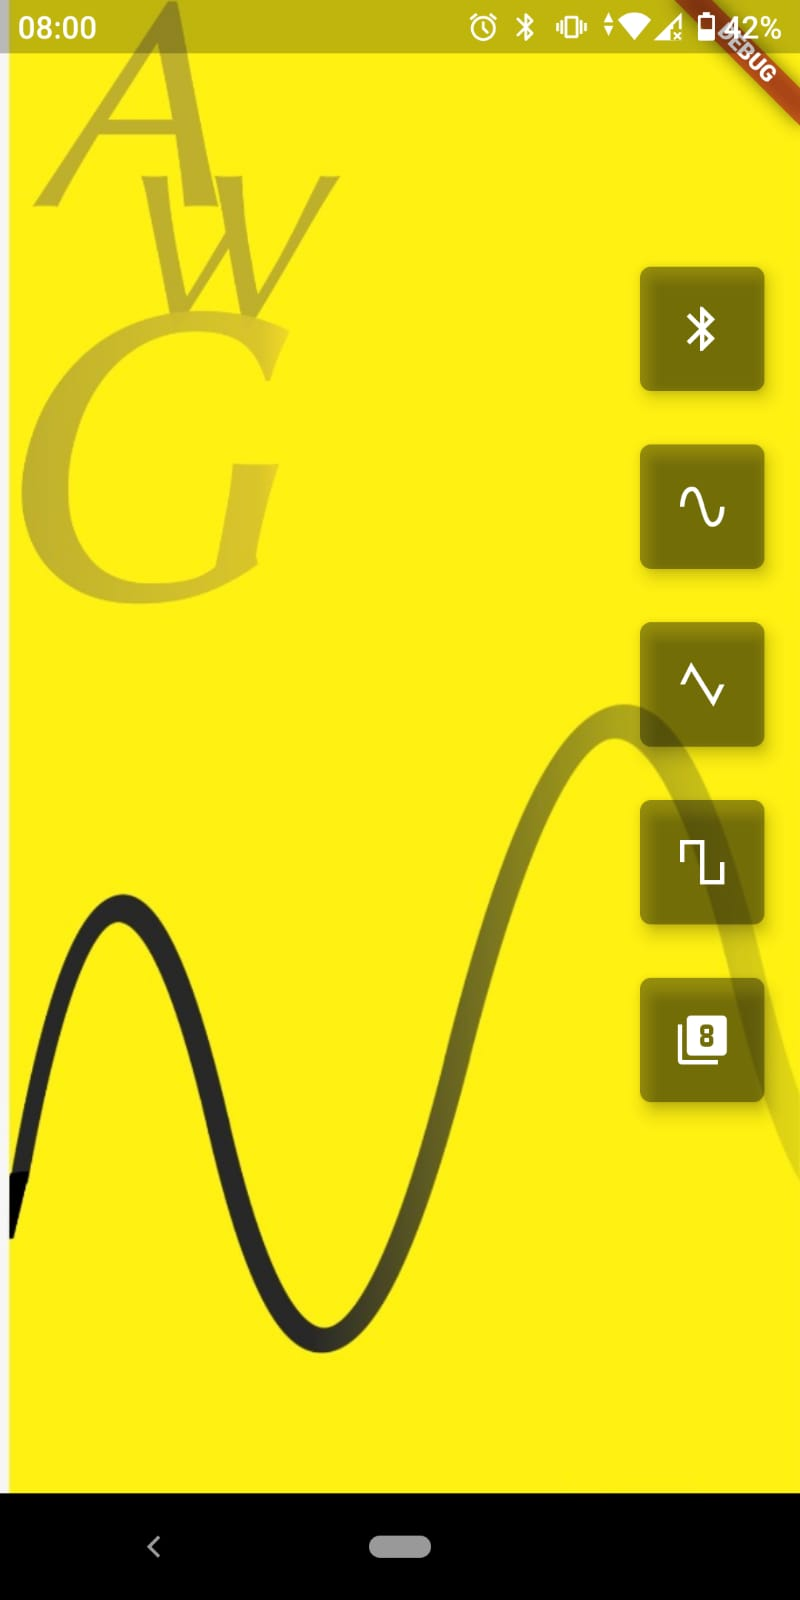
\includegraphics[width=0.4\textwidth]{figs/tela_ini.png}
    \caption{Tela Inicial do \textbf{\nomesoftware{}}}
    \label{fig:telainicial}
\end{figure}

\section{Navegação no Aplicativo}

Embora a tela inicial do aplicativo ofereça um ponto de partida claro para acessar todas as funcionalidades do \textbf{\nomesoftware}, esta seção detalha a navegação entre as diferentes telas e como efetivamente utilizar as ferramentas disponíveis em cada uma delas.

A tela retratada na Figura \ref{fig:bluetooth} leva o usuário às configurações do Bluetooth. Neste ponto o aplicativo necessita de permissões para utilizar o Bluetooth do aparelho, além dos processos de pareamento e conexão com o Raspberry.

\begin{figure}[hbt!]
    \centering    
    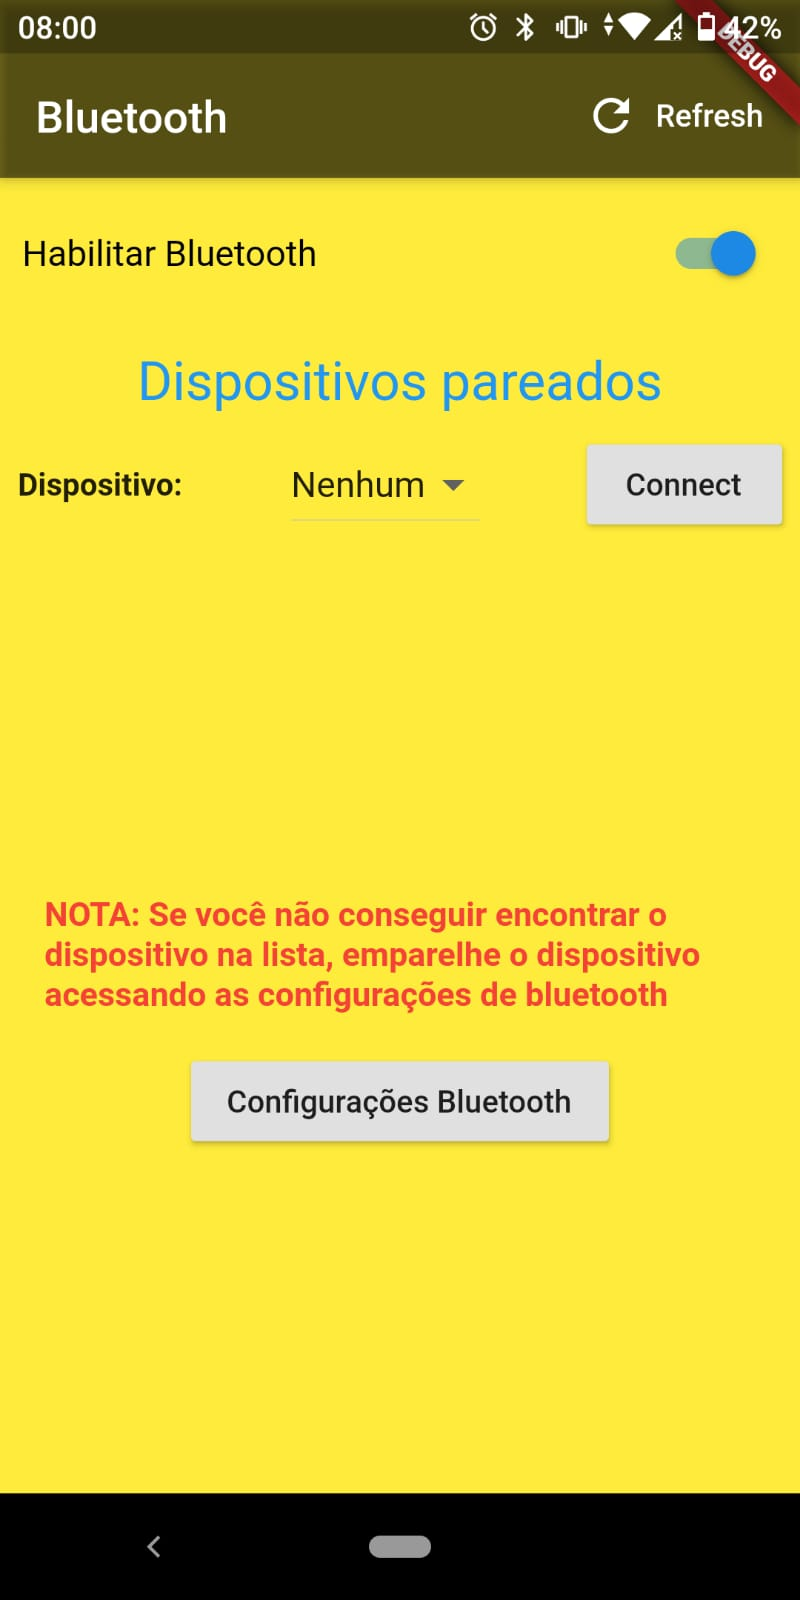
\includegraphics[width=0.4\textwidth]{figs/bt.png}
    \caption{Tela de configuração de \textit{Bluetooth} para conexão com o AWG}
    \label{fig:bluetooth}
\end{figure}

As telas dedicadas a geração dos sinais comuns (senoidal, triangular e quadrado) são muito semelhantes (Figura \ref{fig:sin}, Figura \ref{fig:sq}, Figura \ref{fig:tri}); há campos de entrada de frequência, amplitude, \textit{offset} e, no caso da onda quadrada, \textit{duty cycle}.

\begin{figure}
    \centering
        
    \begin{subfigure}[b]{0.3\textwidth}
        \centering
        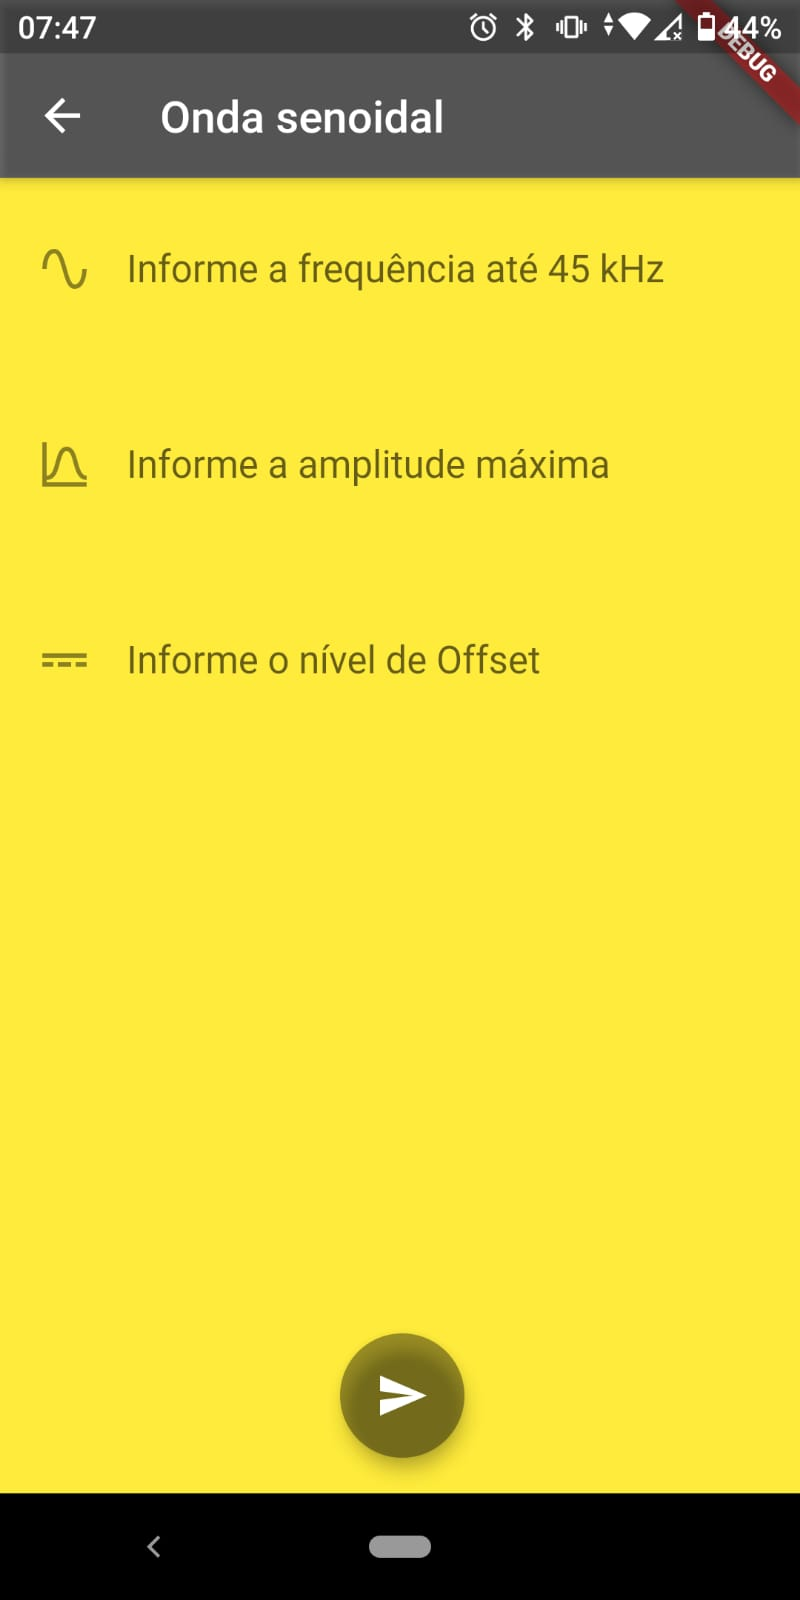
\includegraphics[width=\textwidth]{figs/sin.png}
        \caption{Senoidal}
        \label{fig:sin}
    \end{subfigure}
    %\hfill
    \begin{subfigure}[b]{0.3\textwidth}
        \centering
        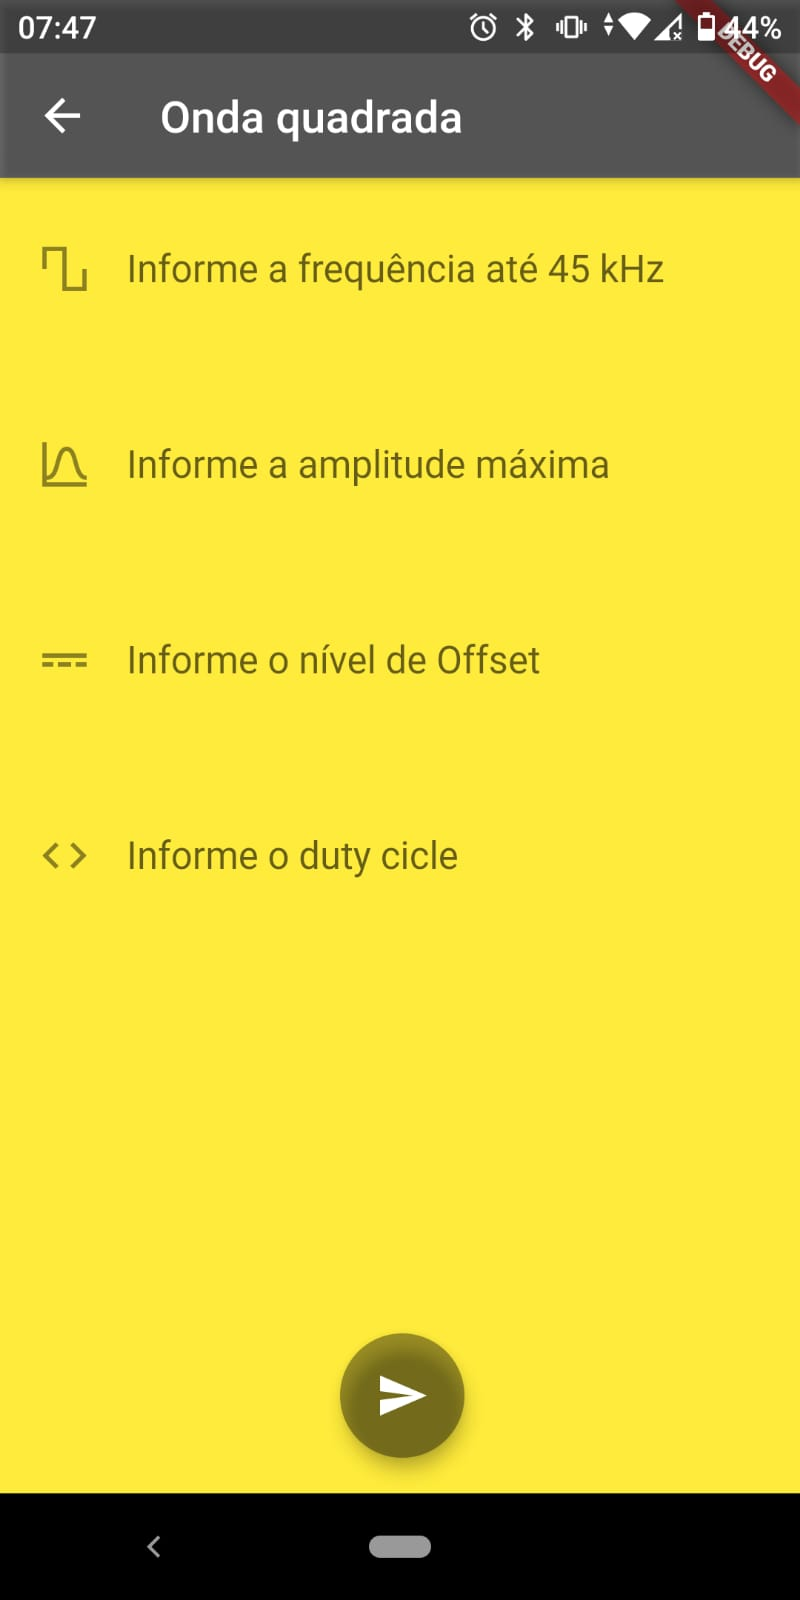
\includegraphics[width=\textwidth]{figs/sq.png}
        \caption{Quadrada}
        \label{fig:sq}
    \end{subfigure}
    %\hfill
    \begin{subfigure}[b]{0.3\textwidth}
        \centering
        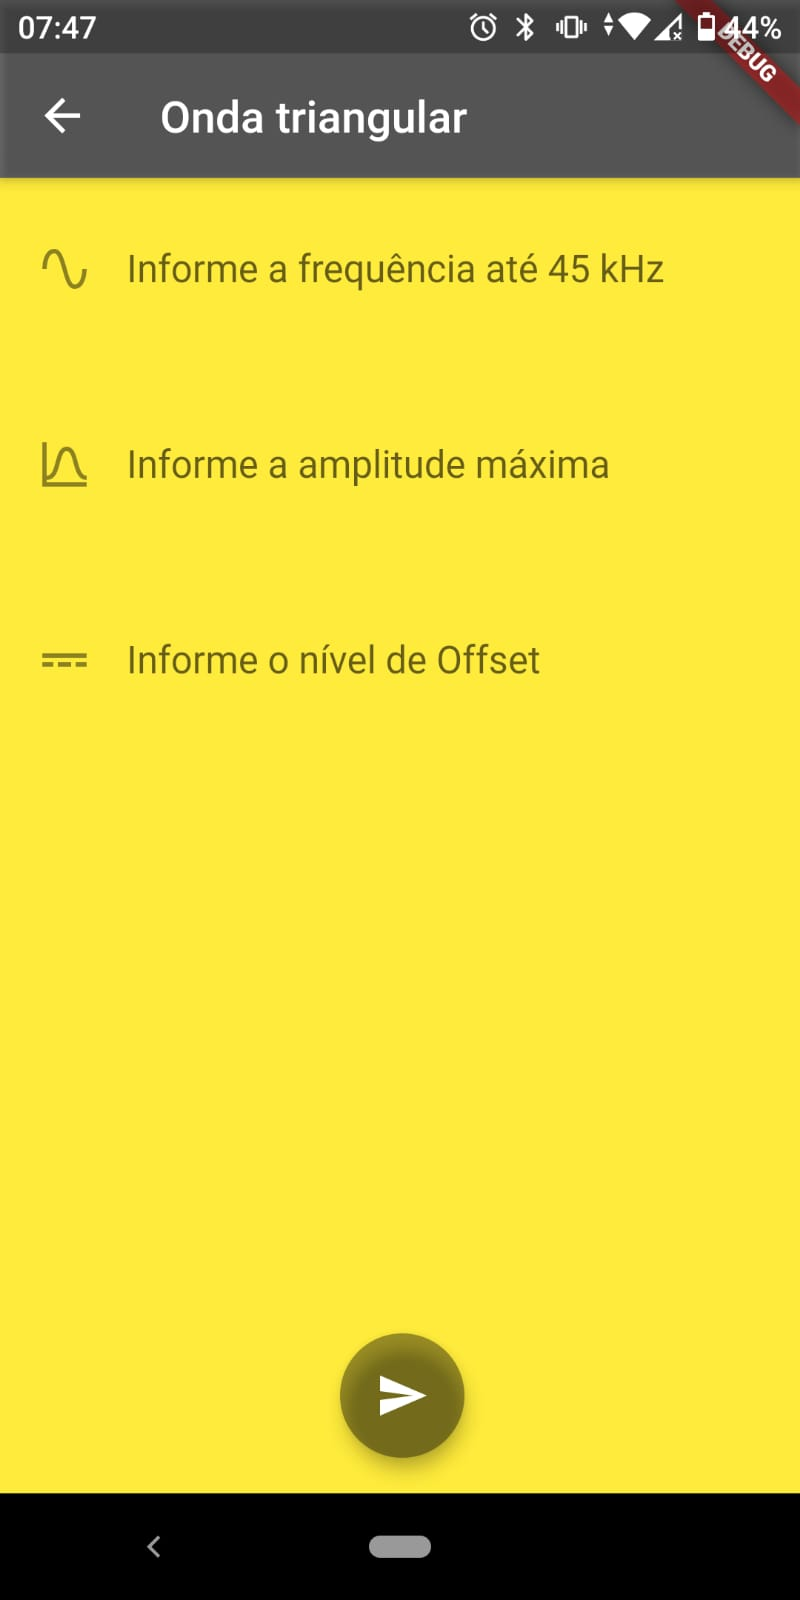
\includegraphics[width=\textwidth]{figs/tri.png}
        \caption{Triangular}
        \label{fig:tri}
    \end{subfigure}

    \caption{Configuração de geração de onda}
    \label{fig:telas app}
\end{figure}

Por fim na Figura \ref{fig:arb} é apresentada a tela dedicada a geração dos sinais arbitrários. Nela é possível digitar os pontos necessários para a sintetização, que devem estar em um intervalo de tempo normalizado entre 0 a 1 e valores de amplitude normalizados entre -1 e 1. Assim, como nas outras telas de configuração de sinal, existem os campos apropriados para configurar frequência, amplitude, \textit{offset}, e neste caso, o tipo de interpolação que será aplicada.

\begin{figure}[hbt!]
    \centering    
    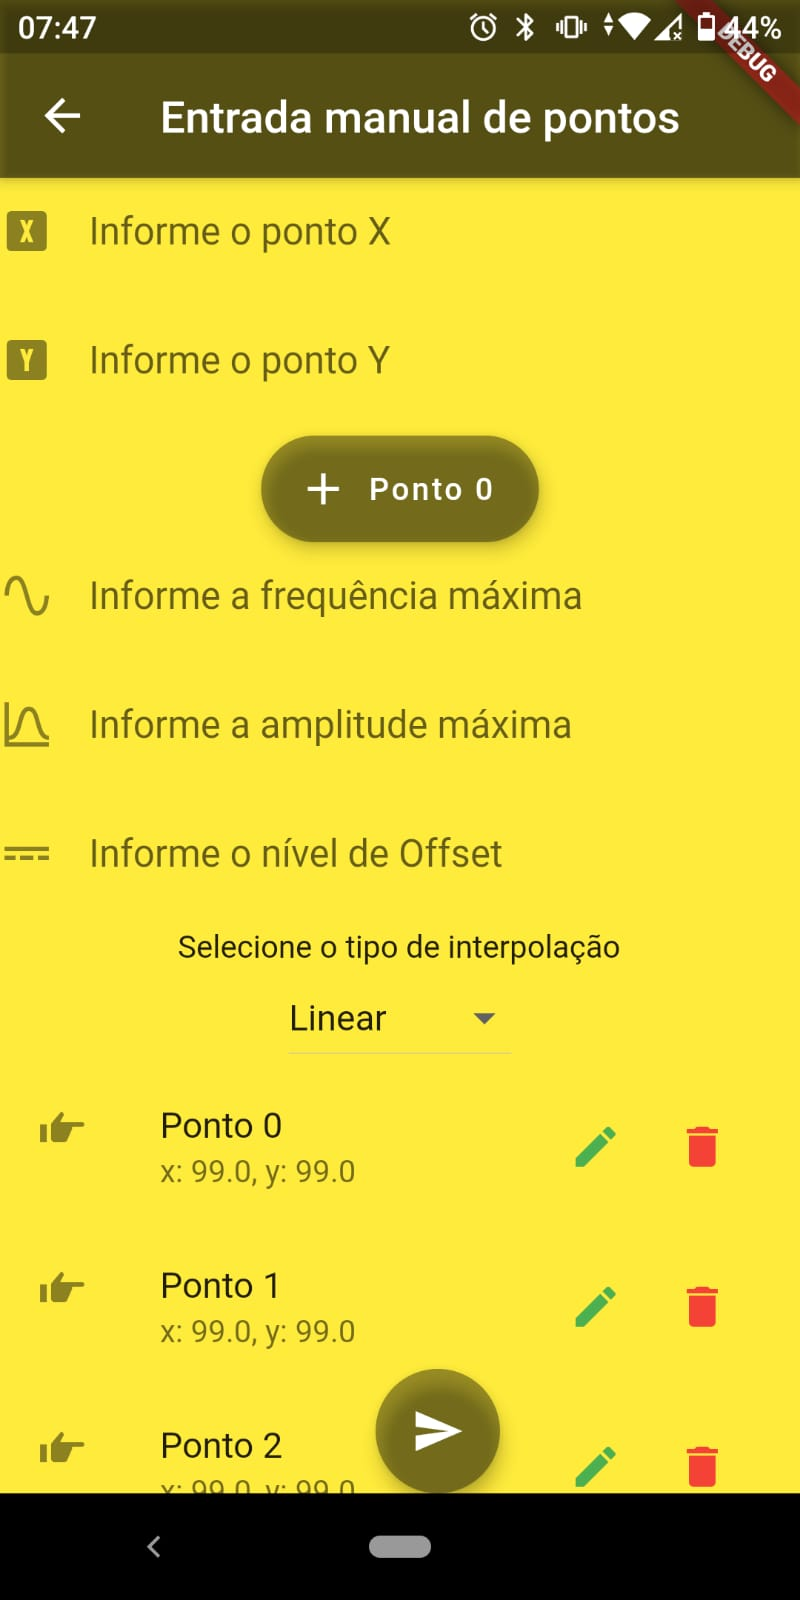
\includegraphics[width=0.4\textwidth]{figs/arb.png}
    \caption{Tela de configuração de sinais arbitrários}
    \label{fig:arb}
\end{figure}


\section{Funcionalidades Específicas}

Aqui, detalhe as funcionalidades específicas do aplicativo, como a geração de formas de onda, controle Bluetooth e manipulação de pontos. Para cada funcionalidade, inclua uma descrição detalhada juntamente com imagens ilustrativas.

% Inserir figuras para cada funcionalidade
\begin{figure}[h]
\centering
%\includegraphics[width=0.6\textwidth]{caminho_para_imagem_funcionalidade_1}
\caption{Funcionalidade 1}
\end{figure}

[...]

\section{Dicas de Uso}

Ofereça dicas para otimizar o uso do aplicativo, incluindo atalhos e recursos menos conhecidos que podem melhorar a experiência do usuário.



Com este guia, você deve ser capaz de navegar e utilizar o \textbf{\nomesoftware{}} com facilidade e eficiência. No próximo capítulo, abordaremos as funcionalidades em detalhes.

\chapter{Funcionalidades do Aplicativo}

O \textbf{\nomesoftware{}} oferece uma variedade de funcionalidades projetadas para facilitar a geração e manipulação de formas de onda, além do controle de dispositivos via Bluetooth. Este capítulo explora cada uma dessas funcionalidades em detalhes.

\section{Geração de Formas de Onda}

O aplicativo permite a geração de várias formas de onda, incluindo ondas triangulares, senoidais e quadradas. Cada tipo de onda pode ser gerado e manipulado de acordo com parâmetros específicos.

\subsection{Onda Triangular}

Descrição de como gerar e manipular ondas triangulares, incluindo ajustes de frequência, amplitude e offset.

% Inserir figura da interface de onda triangular
\begin{figure}[h]
\centering
%\includegraphics[width=0.6\textwidth]{caminho_para_imagem_onda_triangular}
\caption{Geração de Onda Triangular}
\end{figure}

\subsection{Onda Senoidal}

Detalhes sobre a geração de ondas senoidais, com instruções para ajustar as configurações pertinentes.

% Inserir figura da interface de onda senoidal
\begin{figure}[h]
\centering
%\includegraphics[width=0.6\textwidth]{caminho_para_imagem_onda_senoidal}
\caption{Geração de Onda Senoidal}
\end{figure}

\subsection{Onda Quadrada}

Explicação sobre como criar ondas quadradas e como ajustar parâmetros como duty cycle.

% Inserir figura da interface de onda quadrada
\begin{figure}[h]
\centering
%\includegraphics[width=0.6\textwidth]{caminho_para_imagem_onda_quadrada}
\caption{Geração de Onda Quadrada}
\end{figure}

\section{Controle Bluetooth}

Descrição da funcionalidade de controle Bluetooth, incluindo como parear dispositivos, enviar e receber dados.

% Inserir figura da interface Bluetooth
\begin{figure}[h]
\centering
%\includegraphics[width=0.6\textwidth]{caminho_para_imagem_bluetooth}
\caption{Controle Bluetooth}
\end{figure}

\section{Manipulação de Pontos}

Instruções sobre como utilizar a funcionalidade de manipulação de pontos, que permite organizar e analisar dados de forma detalhada.

% Inserir figura da interface de manipulação de pontos
\begin{figure}[h]
\centering
%\includegraphics[width=0.6\textwidth]{caminho_para_imagem_manipulacao_pontos}
\caption{Manipulação de Pontos}
\end{figure}

Este capítulo oferece uma compreensão detalhada das funcionalidades disponíveis no \textbf{\nomesoftware{}}. Com essas informações, você pode explorar e utilizar plenamente as capacidades do aplicativo. No próximo capítulo, abordaremos dicas e técnicas para usuários avançados.

\chapter{Contato e Suporte}

Se você precisar de assistência ou tiver dúvidas relacionadas ao \textbf{\nomesoftware{}}, nossa equipe de suporte está pronta para ajudar. Abaixo estão as informações de contato e os recursos disponíveis para suporte e assistência.

\section{Suporte Técnico}

Para questões técnicas, problemas de funcionamento ou erros no aplicativo, entre em contato com nosso suporte técnico:

\begin{itemize}
    \item Email: suporte@nomedosoftware.com
    \item Telefone: +55 11 1234-5678 (Horário de atendimento: 9h às 18h, de segunda a sexta-feira)
\end{itemize}

\section{Perguntas Frequentes (FAQ)}

Muitas perguntas comuns já têm respostas disponíveis na nossa seção de Perguntas Frequentes. Visite nosso site para acessar o FAQ:

\begin{itemize}
    \item Website: [URL do FAQ no website do software]
\end{itemize}

\section{Fórum da Comunidade}

Para dicas, truques e conselhos de outros usuários do \textbf{\nomesoftware{}}, participe do nosso fórum da comunidade. É um ótimo lugar para compartilhar experiências e aprender com outros entusiastas:

\begin{itemize}
    \item Link do Fórum: [URL do fórum da comunidade]
\end{itemize}

\section{Mídias Sociais}

Siga-nos nas redes sociais para se manter atualizado sobre novidades, dicas e atualizações do \textbf{\nomesoftware{}}:

\begin{itemize}
    \item Facebook: [URL do Facebook]
    \item Twitter: [URL do Twitter]
    \item Instagram: [URL do Instagram]
\end{itemize}

\section{Feedback e Sugestões}

Valorizamos o seu feedback e estamos sempre buscando melhorar o \textbf{\nomesoftware{}}. Se você tiver sugestões ou comentários, por favor, não hesite em nos contatar através do email: feedback@nomedosoftware.com.

Com esses recursos, esperamos que você tenha uma experiência tranquila e satisfatória com o \textbf{\nomesoftware{}}. Lembre-se, estamos aqui para ajudar!


\end{document}
